\section{Background}
\label{sec:background}

\subsection{Blockchain}

At a high level, a blockchain is a sequence of blocks that is immutable in practical applications.
Immutability in blockchains is often provided through Proof of Work.
Proof of Work was introduced in \cite{dwork1992PoW} and first used for blockchain in the Bitcoin whitepaper \cite{nakamoto2009Bitcoin}.
In a Proof of Work blockchain, a block is valid if its cryptographic hash is below a preset threshold.
The threshold is determined by the blockchain community.
It is typically set such that mining a block takes the same amount of time, on average, throughout the life of a blockchain.
The threshold will adapt as blocks are created to meet this requirement.
Each block primarily consists of data that cannot change (financial transactions, medical records, etc).
However, every block contains a field for a fixed-length string of arbitrary bits.
The fixed length string is called a nonce~\cite{nakamoto2009Bitcoin}.
``Mining'' a block consists of searching for a nonce that results in the hash of the block being below the threshold.
By design, it is difficult to find such a nonce because the hash function is cryptographic.
A miner's best strategy is to guess and check nonces until finding a sufficiently low output.
In cryptocurrencies, miners are awarded currency for their work.
Figure \ref{fig:blockchain} displays the typical structure of a blockchain.

\begin{center}
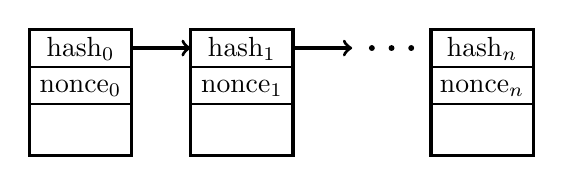
\begin{tikzpicture}[scale=1]

% drawing block 0
\draw [very thick] (0.0,0) rectangle (1.3,1.6);
\draw [white] (0.65,1.35) circle (0.01) node[text=black] {hash$_0$};
\draw [thick] (0.0,1.125) -- (1.3,1.125);
\draw [white] (0.65,0.8500000000000001) circle (0.01) node[text=black] {nonce$_0$};
\draw [thick] (0.0,0.6500000000000001) -- (1.3,0.6500000000000001);
% drawing arrow
\draw [->, very thick] (1.3,1.3625) -- (2.05,1.3625);

% drawing block 1
\draw [very thick] (2.05,0) rectangle (3.3499999999999996,1.6);
\draw [white] (2.6999999999999997,1.35) circle (0.01) node[text=black] {hash$_1$};
\draw [thick] (2.05,1.125) -- (3.3499999999999996,1.125);
\draw [white] (2.6999999999999997,0.8500000000000001) circle (0.01) node[text=black] {nonce$_1$};
\draw [thick] (2.05,0.6500000000000001) -- (3.3499999999999996,0.6500000000000001);
% drawing arrow
\draw [->, very thick] (3.3499999999999996,1.3625) -- (4.1,1.3625);

% draw the dots
\draw [fill=black] (4.35,1.3625) circle (0.03);
\draw [fill=black] (4.6,1.3625) circle (0.03);
\draw [fill=black] (4.85,1.3625) circle (0.03);

% drawing block n
\draw [very thick] (5.1,0) rectangle (6.3999999999999995,1.6);
\draw [white] (5.75,1.35) circle (0.01) node[text=black] {hash$_n$};
\draw [thick] (5.1,1.125) -- (6.3999999999999995,1.125);
\draw [white] (5.75,0.8500000000000001) circle (0.01) node[text=black] {nonce$_n$};
\draw [thick] (5.1,0.6500000000000001) -- (6.3999999999999995,0.6500000000000001);

\end{tikzpicture}
\end{center}

A broader perspective of a blockchain is an implementation of a finite state machine.
In the state machine, blocks are transitions between the states of applications running on top of a blockchain.
Abstractly, the $k^{th}$ block $B_k$ is a transition from state $S_{k-1}$ to state $S_k$ with certain validity requirements.
See Figure \ref{fig:statemachine} for a visual.
A tangible example is a cryptocurrency.
Cryptocurrencies realize state as a record of the amount of currency each public key controls.
Blocks are a set of transactions that transfer currency between public keys (analogous to accounts).
In state $S_0$, no one controls any currency.
Then block $B_1$ is created and its miner is granted some currency.
This moves the blockchain to $S_1$ which records how much currency that miner controls.
Then block $B_2$ is mined, granting cryptocurrency to its miner.
Additionally, block $B_2$ could contain a currency transfer from the miner of the first block to another user.
Then the state $S_2$ records how much funds each user of the cryptocurreny controls.
Then block $B_3$ is created and the sate machine is updated with the changes in ``account'' balances.
This process repeats until state $S_n$ is reached, which contains the current account-balance pairs of all the current users of a cryptocurrency.

\begin{center}
    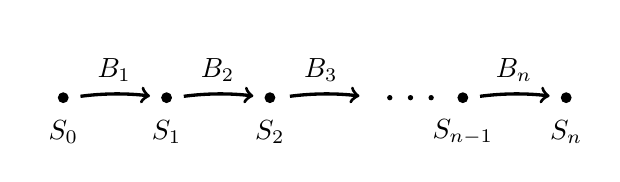
\begin{tikzpicture}[scale=1.75]
        % draw the 0 point
        \draw [thick,color=white] (0,0) -- (0,0);

        % state 0
        \draw [fill=black] (0.25,-0.5) circle (0.035);
        \node at (0.25,-0.75) {$S_0$};

        % block 1
        \draw [very thick, ->] (0.375,-0.49) arc (97.5:83:2);
        \node at (0.62,-0.3) {$B_1$};

        % state 1
        \draw [fill=black] (1,-0.5) circle (0.035);
        \node at (1,-0.75) {$S_1$};

        % block 2
        \draw [very thick, ->] (1.125,-0.49) arc (97.5:83:2);
        \node at (1.37,-0.3) {$B_2$};

        % state 2
        \draw [fill=black] (1.75,-0.5) circle (0.035);
        \node at (1.75,-0.75) {$S_2$};

        % block 3
        \draw [very thick, ->] (1.895,-0.49) arc (97.5:83:2);
        \node at (2.12,-0.3) {$B_3$};

        % ...
        \draw [fill=black] (2.62,-0.5) circle (0.015);
        \draw [fill=black] (2.77,-0.5) circle (0.015);
        \draw [fill=black] (2.92,-0.5) circle (0.015);

        % state n-1
        \draw [fill=black] (3.15,-0.5) circle (0.035);
        \node at (3.15,-0.75) {$S_{n-1}$};

        % block n
        \draw [very thick, ->] (3.275,-0.49) arc (97.5:83:2);
        \node at (3.52,-0.3) {$B_n$};

        % state n
        \draw [fill=black] (3.90,-0.5) circle (0.035);
        \node at (3.90,-0.75) {$S_n$};

    \end{tikzpicture}
    \captionof{figure}{Blocks as transitions between states \label{fig:statemachine}}
\end{center}


\subsection{Technical Problem}

To understand the technical problem, we must understand two properties of blockchains.
First, miners must obtain every block before mining new blocks.
And, second, blockchains grow in perpetuity.
These properties mean that new miners must download and process an ever increasing amount of data as time passes.
Even now, when Bitcoin is just over a decade old, it can take days to become a miner. % maybe cite Bernardini but they have no source for that claim
Such a barrier can deter large machines from the joining the chain and entirely prevent small machines from mining.

The root of the problem is that mining requires all the information in a blockchain.
Our goal is to produce an off-chain, efficient, and secure method to bootstrap miners in a blockchain.
An off-chain solution is one that does affect the underlying blockchain.
This is important because many on-chain solutions to this problem cause a hard fork in a blockchain.
A hard fork is when a blockchain splits because miners disagree on the format of a block~\cite{lin2017Survey}.
While a blockchain can survive a hard fork, the mining power splits and weakens the blockchain.
We want an efficient solution so that our idea could be useful in an actual blockchain.
Finally, security is important because blockchains often record important information such as medical records. 
Our solution should not introduce vulnerabilities to such important information.

To frame this project, we use the Goal Question Metric approach presented in \cite{basili1994goal}.
This results in ``the specification of a measurement system targeting a particular set of issues and a set of rules for the interpretation of the measurement data \cite{basili1994goal}.''
The model has three levels.
At the conceptual level, a goal is defined.
A goal consists of a purpose, an issue, a process, and a viewpoint.
At the operational level, a set of questions are asked that characterizes the goal.
At the quantitative level, data is associated with questions in an attempt to answer them.
The data can be either objective or subjective.
Table \ref{tab:gqm} displays the Goal Question Metric Approach we will use for this project.

\newpage 

\begin{center}
	\vspace{1em}
    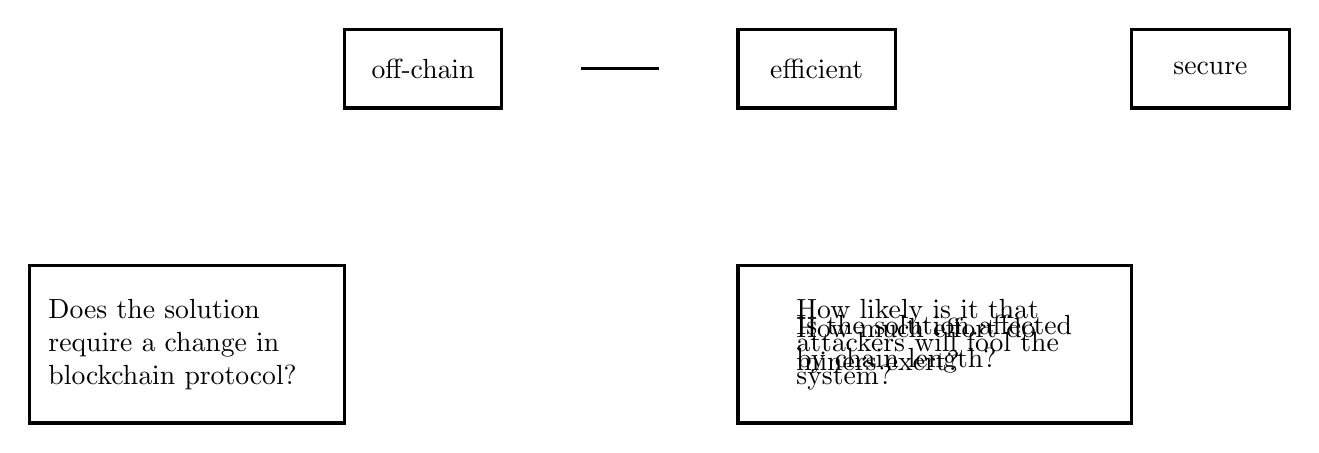
\begin{tikzpicture}
    % GQM hierarchy

    % goals
    \draw [very thick] (0,0) rectangle (2,-1) node[midway] {off-chain};
    \draw [very thick] (5,0) rectangle (7,-1) node[midway] {efficient};
    \draw [very thick] (10,0) rectangle (12,-1) node[midway] {secure};

    % questions
    \draw [very thick] (-4,-3) rectangle (0,-5) node[midway,text width=100] {{\singlespacing Does the solution require a change in blockchain protocol?}};
    \draw [very thick] (5,-3) rectangle (10,-5) node[midway,text width=100] {Is the solution affected by chain length?};
    \draw [very thick] (5,-3) rectangle (10,-5) node[midway,text width=100] {How much effort do miners exert?};
    \draw [very thick] (5,-3) rectangle (10,-5) node[midway,text width=100] {How likely is it that attackers will fool the system?};

    % lines (length 0.75)
    \draw [very thick] (3,-0.5) -- (4,-0.5);

    \end{tikzpicture}
    \captionof{figure}{Goal Question Metric hierarchy \label{fig:gqm}}
\end{center}


\subsection{Related Work}

Truncating the required bootstrapping information in a blockchain is an active area of research.
The remainder of Section \ref{sec:background} is devoted to summarizing existing ideas and solutions.

% lightweight nodes in the bitcoin whitepaper

The Bitcoin whitepaper~\cite{nakamoto2009Bitcoin} introduces the concept of lightweight nodes.
Instead of becoming a full node, lightweight nodes only store the header chain and query full nodes to see if transactions are valid.
This is a step in the right direction because the header chain downloads quickly, but it does not grant nodes the ability to mine new blocks.
Nodes can only verify old transactions.

% summary block in the main chain

Another idea is to periodically place a summary block in the original blockchain~\cite{palai2018BlockSummariesSameChain}~\cite{nadiya2018BlockSummaries(ExtendsPalai)}.
A summary block is responsible for reporting the net change caused by a certain amount of previous blocks.
This process can be made recursive to any depth by creating a summary block responsible for a set of summary blocks (a summary of summaries)~\cite{palai2018BlockSummariesSameChain}~\cite{nadiya2018BlockSummaries(ExtendsPalai)}.
Trust in the summary blocks is built in the same fashion as trust in the regular blockchain.
A node joining the network would download the header chain and relevant summary blocks.
If a summary block has been accounted for by another summary block, there is no need to download it.
This idea is nice because it relies on the same security principles as blockchain, but the implementation would require a hard fork.

% miniblockchain

A different idea would be to use mini-blockchain~\cite{bruce2014Miniblockchain}.
A mini-blockchain requires that a block $B_k$ includes the hash of $S_k$, cryptographically tying the state to the blockchain.
A bootstrapping node can then request the header chain, a recent state, and blocks following the recent state.
The new node can verify that the received state corresponds with the blockchain and then compute the current state with the information in the newest blocks.
While this solution is quite clean, it would cause a hard fork.

% separate summary chain

Another way to provide state would be to create a new blockchain that records state~\cite{marsalek2019BockSummariesSeparateChain}.
The new blockchain records the state of the original chain every so often and bootstrapping nodes can eliminate the need for blocks prior to the most recent summary.
Since each state exists independently of all other states, the size of the second blockchain will not bloat like the original chain~\cite{marsalek2019BockSummariesSeparateChain}.
While this solution does operate off-chain, it is not necessarily secure.
It is unlikely that a miner will give up valuable computing power to contribute to the second blockchain.
This could allow a powerful, malicious actor to sabotage the second blockchain, making it unreliable.

% coinprune

The final related idea holds an election to verify state~\cite{matzutt2020HowTSPrune}.
Miners are allowed to vote for a state and then bootstrapping nodes trust the majority of votes.
Each vote is recorded in a block and each block has the capacity to store a single vote~\cite{matzutt2020HowTSPrune}.
Storing votes in blocks makes them immutable, so a bootstrapping node is able to collect every vote.
The issues with this idea are two-fold.
First, a vote can only be generated as quickly as new blocks.
In Bitcoin, this averages to about 10 minutes per block~\cite{nakamoto2009Bitcoin}, meaning a bootstrapping node might have to wait a week for there to be sufficiently many votes to trust a state.
Second, \cite{matzutt2020HowTSPrune} relies on implementation details in the Bitcoin protocol and does not apply to blockchains in general.
